\documentclass[14pt]{extarticle}

\usepackage[table]{xcolor} % colored lines for tables
%\usepackage[normalem]{ulem} % strike through text
\usepackage{amsmath,mathtools,amsfonts,amsthm,amssymb,hyperref,mathrsfs}
\usepackage{parskip,geometry,latexsym,bookmark,mathtools,float,cancel}
%\usepackage{tcolorbox,bm}

\newtheorem{defn}{Definition}
\newtheorem{thm}{Theorem}
\newtheorem{claim}{Claim}
\newtheorem{lemma}{Lemma}

\newcommand{\dps}{\displaystyle}
\newcommand{\es}{\varnothing}
\newcommand{\fbl}{\underline{\hspace{1cm}}\,\,}
\newcommand{\R}{\mathbb{R}}
\newcommand{\Q}{\mathbb{Q}}
\newcommand{\Z}{\mathbb{Z}}
\newcommand{\from}{\leftarrow}
\newcommand{\true}{{\bf t}}
\newcommand{\false}{{\bf c}}
\newcommand{\bic}{\leftrightarrow}
\newcommand{\da}{\downarrow}
\newcommand{\fa}{\forall}
\newcommand{\te}{\exists}
\newcommand{\cy}{\color{cyan}}

\newcommand{\colsq}[1]{{\color{#1} $\blacksquare$}}

\newcommand{\base}[1]{{\cy #1}} % for log bases
\newcommand{\floor}[1]{{\left\lfloor#1\right\rfloor}}
\newcommand{\ceil}[1]{{\left\lceil#1\right\rceil}}
\newcommand\Ccancel[2][black]{\renewcommand\CancelColor{\color{#1}}\cancel{#2}}
\newcommand\Cbcancel[2][black]{\renewcommand\CancelColor{\color{#1}}\bcancel{#2}}

%\renewcommand{\arraystretch}{1.2}
%\setlength{\extrarowheight}{10pt}

\hypersetup{colorlinks,allcolors=blue,linktoc=all}
\geometry{a4paper}
\geometry{margin=0.42in}

\title{Chapter 12 Solutions, Susanna Epp Discrete Math 5th Edition}

\author{https://github.com/spamegg1}

\begin{document}
\maketitle
\tableofcontents

\section{Exercise Set 12.1}

{\bf \cy In 1 and 2, let \(\Sigma = \{x, y\}\) be an alphabet.}

\subsection{Exercise 1}
\subsubsection{(a)}
Let \(L_1\) be the language consisting of all strings over \(\Sigma\) that are palindromes and have length \(\leq 4\). 
List the elements of \(L_1\) between braces.

\begin{proof}
\(L_1 = \{\lambda, x, y, xx, yy, xxx, xyx, yxy, yyy, xxxx, xyyx, yxxy, yyyy\}\)
\end{proof}

\subsubsection{(b)}
Let \(L_2\) be the language consisting of all strings over \(\Sigma\) that begin with an \(x\) and have length \(\leq 3\). 
List the elements of \(L_2\).

\begin{proof}
\(L_2 = \{x, xx, xy, xxx, xxy, xyx, xyy\}\)
\end{proof}

\subsection{Exercise 2}
\subsubsection{(a)}
Let \(L_3\) be the language consisting of all strings over \(\Sigma\) of length \(\leq 3\) in which all the \(x\)’s appear 
to the left of all the \(y\)’s. List the elements of \(L_3\) between braces.

\begin{proof}
\(L_3 = \{\lambda, x, y, xx, xy, yy, xxx, xxy, xyy, yyy\}\)
\end{proof}

\subsubsection{(b)}
List between braces the elements of \(\Sigma^4\), the set of all strings of length 4 over \(\Sigma\).

\begin{proof}
\(L_4 = \{xxxx, xxxy, xxyx, xxyy, xyxx, xyxy, xyyx, xyyy, yxxx, yxxy, yxyx, yxyy,\) \\
\(yyxx, yyxy, yyyx, yyyy\}\)
\end{proof}

\subsubsection{(c)}
Let \(A = \Sigma^1 \cup \Sigma^2\) and \(B = \Sigma^3 \cup \Sigma^4\). Describe \(A, B\), and \(A \cup B\) in words.

\begin{proof}
\(A\) is the set of strings over \(\Sigma\) of length 1 or 2.
\(B\) is the set of strings over \(\Sigma\) of length 3 or 4.
\(A \cup B\) is the set of strings over \(\Sigma\) of length 1 or 2 or 3 or 4.
\end{proof}

\subsection{Exercise 3}
\subsubsection{(a)}
If the expression \(ab + cd + \cdot\) in postfix notation is converted to infix notation, what is the result?

\begin{proof}
\((a + b)\cdot(c + d)\)
\end{proof}

\subsubsection{(b)}
Let \(\Sigma = \{1, 2, *, /\}\) and let \(L\) be the set of all strings over \(\Sigma\) obtained by writing first a number 
(1 or 2), then a second number (1 or 2), which can be the same as the first one, and finally an operation (denoted * or /, 
where * indicates multiplication and / indicates division). Then \(L\) is a set of postfix, or reverse Polish, 
expressions. List all the elements of \(L\) between braces, and evaluate the resulting expressions.

\begin{proof}
\(L = \{11*, 11/, 12*, 12/, 21*, 21/, 22*, 22/\}\) These evaluate to: \\
\(1 \cdot 1 = 1, 1 / 1 = 1, 1 \cdot 2 = 2, 1 / 2 = \frac{1}{2}, 2 \cdot 1 = 2, 2 / 1 = 2, 2 \cdot 2 = 4, 2 / 2 = 1\).
\end{proof}

{\bf \cy In \(4-6\), describe \(L_1L_2\), \(L_1 \cup L_2\), and \((L_1 \cup L_2)^*\) for the given languages \(L_1\) and 
\(L_2\).}

\subsection{Exercise 4}
\(L_1\) is the set of all strings of \(a\)’s and \(b\)’s that start with an \(a\) and contain only that one \(a\); \(L_2\) 
is the set of all strings of \(a\)’s and \(b\)’s that contain an even number of \(a\)’s.

\begin{proof}
\(L_1L_2\) is the set of all strings of \(a\)’s and \(b\)’s that start with an \(a\) and contain an odd number of \(a\)’s. 
\(L_1 \cup L_2\) is the set of all strings of \(a\)’s and \(b\)’s that contain an even number of \(a\)’s or that start 
with an \(a\) and contain only that one \(a\). (Note that because 0 is an even number, both \(\lambda\) and \(b\) are in 
\(L_1 \cup L_2\).) \((L_1 \cup L_2)^*\) is the set of all strings of \(a\)’s and \(b\)’s. The reason is that \(a\) and 
\(b\) are both in \(L_1 \cup L_2\), and thus every string in \(a\) and \(b\) is in \((L_1 \cup L_2)^*\).
\end{proof}

\subsection{Exercise 5}
\(L_1\) is the set of all strings of \(a\)’s, \(b\)’s, and \(c\)’s that contain no \(c\)’s and have the same number of 
\(a\)’s as \(b\)’s; \(L_2\) is the set of all strings of \(a\)’s, \(b\)’s, and \(c\)’s that contain no \(a\)’s or 
\(b\)’s.

\begin{proof}
Note that \(\lambda \in L_1\) since 0 is a number and \(\lambda\) contains the same number of, namely 0 of, \(a\)'s
and \(b\)'s, and contains no \(c\)'s. Similarly \(\lambda \in L_2\) because \(\lambda\) contains no \(a\)'s or \(b\)'s.

\(L_1L_2\) is the set of all strings of \(a\)’s, \(b\)’s and \(c\)’s that contain the same number of \(a\)’s and \(b\)’s,
where all the \(c\)'s are to the right of all \(a\)’s and \(b\)’s. Since \(\lambda \in L_1\) and \(\lambda \in L_2\),
\(\lambda \in L_1L_2\) too, and moreover \(L_1 \subseteq L_1L_2\) (due to \(l_1 \lambda\) for all \(l_1 \in L_1\)) and 
\(L_2 \subseteq L_1L_2\) (due to \(\lambda l_2\) for all \(l_2 \in L_2\)).

\(L_1 \cup L_2\) is the set of all strings of \(a\)’s, \(b\)’s and \(c\)’s that either contain the same number of \(a\)’s and 
\(b\)’s and no \(c\)'s, or contain no \(a\)'s or \(b\)'s. 

\((L_1 \cup L_2)^*\) is the set of all strings of \(a\)’s, \(b\)’s and \(c\)’s that contain the same number of \(a\)’s and 
\(b\)’s.
\end{proof}

\subsection{Exercise 6}
\(L_1\) is the set of all strings of 0’s and 1’s that start with a 0; \(L_2\) is the set of all strings of 0’s and 1’s 
that end with a 0.

\begin{proof}
\(L_1L_2\) is the set of all strings of 0’s and 1’s that start with a 0 and end with a 0. (\(\lambda\) not included.)

\(L_1 \cup L_2\) is the set of all strings of 0’s and 1’s that either start with a 0, or end with a 0 (or both). 
(\(\lambda\) not included.)

\((L_1 \cup L_2)^*\) is the set of all strings of 0’s and 1’s that either start with a 0, or end with a 0, including
\(\lambda\).
\end{proof}

{\bf \cy In \(7-9\), add parentheses to emphasize the order of precedence in the given expressions.}

\subsection{Exercise 7}
\((a | b^*b)(a^* | ab)\)

\begin{proof}
\((a | ((b^*)b))((a^*) | (ab))\)
\end{proof}

\subsection{Exercise 8}
\(0^*1 | 0(0^*1)^*\)

\begin{proof}
\(((0^*)1) | (0(((0^*)1)^*))\)
\end{proof}

\subsection{Exercise 9}
\((x | yz^*)^*(yx | (yz)^*z)\)

\begin{proof}
\(((x | (y(z^*)))^*) ((yx) | (((yz)^*)z))\)
\end{proof}

{\bf \cy In \(10-12\), use the rules about order of precedence to eliminate the parentheses in the given regular expression.}

\subsection{Exercise 10}
\(((a(b^*)) | (c(b^*))) ((ac) | (bc))\)

\begin{proof}
\((ab^* | cb^*)(ac | bc)\)
\end{proof}

\subsection{Exercise 11}
\((1(1^*)) | ((1(0^*)) | ((1^*)1))\)

\begin{proof}
\(11^* | (10^* | 1^*1)\)
\end{proof}

\subsection{Exercise 12}
\((xy)(((x^*)y)^*) | (((yx) | y)(y^*))\)

\begin{proof}
\(xy(x^*y)^* | (yx | y)y^*\)
\end{proof}

{\bf In \(13-15\), use set notation to derive the language defined by the given regular expression. 
Assume \(\Sigma = \{a, b, c\}\).}

\subsection{Exercise 13}
\(\lambda | ab\)

\begin{proof}
\(L(\lambda | ab) = L(\lambda) \cup L(ab) = \{\lambda\} \cup L(a)L(b) = \{\lambda\} \cup \{xy \,|\, x \in L(a) \text{ and } 
y \in L(b)\} = \{\lambda\} \cup \{xy \,|\, x \in \{a\} \text{ and } y \in \{b\}\} = \{\lambda\} \cup \{ab\} = 
\{\lambda, ab\}\)
\end{proof}

\subsection{Exercise 14}
\(\es | \lambda\)

\begin{proof}
\(L(\es | \lambda) = L(\es) \cup L(\lambda) = \es \cup \{\lambda\} = \{\lambda\}\)
\end{proof}

\subsection{Exercise 15}
\((a | b)c\)

\begin{proof}
\(L((a | b)c) = L(a|b)L(c) = (L(a) \cup L(b))L(c) = (\{a\} \cup \{b\})\{c\} = \{a,b\}\{c\} = \{xy \, | \, x \in \{a,b\} 
\text{ and } y \in \{c\}\} = \{ac, bc\}\)
\end{proof}

{\bf \cy In 16–18, write five strings that belong to the language defined by the given regular expression.}

\subsection{Exercise 16}
\(0^*1(0^*1^*)^*\)

\begin{proof}
Here is a sample of five strings out of infinitely many: 0101, 1, 01, 10000, and 011100.
\end{proof}

\subsection{Exercise 17}
\(b^* | b^*ab^*\)

\begin{proof}
\(b, a, bab, babb, bbab\)
\end{proof}

\subsection{Exercise 18}
\(x^*(yxxy | x)^*\)

\begin{proof}
\(yxxy, yxxyyxxy, xyxxy, xx, xxyxxyxx\)
\end{proof}

{\bf In \(19-21\), use words to describe the language defined by the given regular expression.}

\subsection{Exercise 19}
\(b^*ab^*ab^*a\)

\begin{proof}
The language consists of all strings of \(a\)’s and \(b\)’s that contain exactly three \(a\)’s and end in an \(a\).
\end{proof}

\subsection{Exercise 20}
\(1(0 | 1)^* 00\)

\begin{proof}
All strings that begin with a 1 and end in 00.
\end{proof}

\subsection{Exercise 21}
\((x | y)y(x | y)^*\)

\begin{proof}
All strings that start with either \(xy\) or \(yy\), then followed by any string made up of \(x\)'s and \(y\)'s.
\end{proof}

{\bf \cy In \(22-24\), indicate whether the given strings belong to the language defined by the given regular 
expression. Briefly justify your answers.}

\subsection{Exercise 22}
Expression: \((b | l)a(a | b)* a(b | l)\), strings: \(aaaba, baabb\)

\begin{proof}
\(aaaba\) is in the language but \(baabb\) is not because if a string in the language contains a \(b\) to the right of the 
left-most \(a\), then it must contain another \(a\) to the right of all the \(b\)’s.
\end{proof}

\subsection{Exercise 23}
Expression: \((x^*y | zy^*)^*\), strings: \(zyyxz, zyyzy\)

\begin{proof}
\(zyyxz\) is not in the language because, due to the rule \(x^*y\) being the only rule that includes an \(x\), the last
\(x\) in a string must be followed by a \(y\).

\(zyyzy\) is in the language because, \(zyy\) can be obtained from \(zy^*\), then \(zy\) can also be obtained from \(zy^*\),
and they can be concatenated due to the outer \(^*\).
\end{proof}

\subsection{Exercise 24}
Expression: \((01^*2)^*\), strings: 120, 01202

\begin{proof}
120 is not in the language because, every nonempty string must contain a 0 at the start.

01202 is in the language because, \(012\) can be obtained from \(01^*2\), then \(02\) can also be obtained from \(01^*2\), 
then they can be concatenated due to the outer \(^*\).
\end{proof}

{\bf \cy In \(25-27\), find a regular expression that defines the given language.}

\subsection{Exercise 25}
The language consisting of all strings of 0’s and 1’s with an odd number of 1’s. (Such a string is said to have odd parity.)

\begin{proof}
One solution is \(0^*10^*(0^*10^*10^*)^*\).
\end{proof}

\subsection{Exercise 26}
The language consisting of all strings of \(a\)’s and \(b\)’s in which the third character from the end is a \(b\).

\begin{proof}
One solution is \((a|b)^*b(aa|ab|ba|bb)\).
\end{proof}

\subsection{Exercise 27}
The language consisting of strings of \(x\)’s and \(y\)’s in which the elements in every pair of \(x\)’s are separated by 
at least one \(y\).

\begin{proof}
We can think of the string as follows: start with 0 or more \(y\)'s, followed by one \(x\) and one \(y\) (because two 
\(x\)`s cannot be next to each other) and 0 or more \(y\)'s,
which can be repeated as many times, then finally followed by
either \(\lambda\) or one \(x\).

So one solution is \(y^*(xyy^*)^*(\lambda | x)\).
\end{proof}

{\bf \cy Let \(r\), \(s\), and \(t\) be regular expressions over \(\Sigma = \{a, b\}\). In \(28-30\), determine whether 
the two regular expressions define the same language. If they do, describe the language. If they do not, give an example of 
a string that is in one of the languages but not the other.}

\subsection{Exercise 28}
\((r | s)t\) and \(rt | st\)

\begin{proof}
\(L((r | s)t) = L(r | s)L(t) = (L(r) \cup L(s))L(t)\) \\
\(= \{xy | (x \in L(r) \cup L(s)) \text{ and } y \in L(t)\}
= \{xy | (x \in L(r) \text{ or } x \in L(s)) \text{ and } y 
\in L(t)\}\) \\
\(= \{xy | (x \in L(r) \text{ and } y \in L(t)) \text{ or } (x \in L(s) \text{ and } y \in L(t))\}\) \\
\(= \{xy | xy \in L(rt) \text{ or } xy \in L(st)\} = L(rt) \cup L(st) = L(rt | st)\)

The language can be described as: \(\{xy \, | \, x \in L(r) \cup L(s) \text{ and } y \in L(t)\}\).
\end{proof}

\subsection{Exercise 29}
\((rs)^*\) and \(r^*s^*\)

\begin{proof}
The string \(rr\) is in the second language but not in the first language.
\end{proof}

\subsection{Exercise 30}
\((rs)^*\) and \(((rs)^*)^*\)

\begin{proof}
\((rs)^* = \{\lambda, rs, rsrs, rsrsrs, rsrsrsrs, \ldots\}\) and \\
\(((rs)^*)^* = \{\lambda, rs, rsrs, rsrsrs, rsrsrsrs, \ldots\}^* = \{\lambda, rs, rsrs, rsrsrs, rsrsrsrs, \ldots\}\).

The two expressions define the same language. It can be described as: the set of strings that are 0 or more 
occurrences of \(rs\) concatenated.
\end{proof}

{\bf \cy In \(31-39\), write a regular expression to define the given set of strings. Use the shorthand notations given in 
the section whenever convenient. In most cases, your expression will describe other strings in addition to the 
given ones, but try to make your answer fit the given strings as closely as possible within reasonable space limitations.}

\subsection{Exercise 31}
All words that are written in lowercase letters and start with the letters \(pre\) but do not consist of \(pre\) all by 
itself.

\begin{proof}
\(pre[a - z]^+\)
\end{proof}

\subsection{Exercise 32}
All words that are written in uppercase letters, and contain the letters \(BIO\) (as a unit) or \(INFO\) (as a unit).

\begin{proof}
\([A-Z]^*(BIO | INFO)[A-Z]^*\)
\end{proof}

\subsection{Exercise 33}
All words that are written in lowercase letters, end in \(ly\), and contain at least five letters.

\begin{proof}
\([a-z]^+[a-z]^+[a-z]^+ ly\)
\end{proof}

\subsection{Exercise 34}
All words that are written in lowercase letters and contain at least one of the vowels a, e, i, o, or u.

\begin{proof}
\([a - z]^*(a | e | i | o | u)[a - z]^*\)
\end{proof}

\subsection{Exercise 35}
All words that are written in lowercase letters and contain exactly one of the vowels a, e, i, o, or u.

\begin{proof}
\([\string^ aeiou]^*(a|e|i|o|u)[\string^ aeiou]^*\). Here \(\string^ aeiou\) means  all the letters except those five: 
\(bcdfghjklmnpqrstvwxyz\).
\end{proof}

\subsection{Exercise 36}
All words that are written in uppercase letters and do not start with one of the vowels A, E, I, O, or U but contain 
exactly two of these vowels next to each other.

\begin{proof}
\([\string^ AEIOU][A-Z]^*[AEIOU]\{2\}[A-Z]^*\)
\end{proof}

\subsection{Exercise 37}
All United States social security numbers (which consist of three digits, a hyphen, two digits, another hyphen, and 
finally four more digits), where the final four digits start with a 3 and end with a 6.

\begin{proof}
\([0 - 9]\{3\} - [0 - 9]\{2\} - 3[0 - 9]\{2\}6\)
\end{proof}

\subsection{Exercise 38}
All telephone numbers that have three digits, then a hyphen, then three more digits, then a hyphen, and then four digits, 
where the first three digits are either 800 or 888 and the last four digits start and end with a 2.

\begin{proof}
\((800|888)-[0-9]\{3\}-2[0-9]\{2\}2\)
\end{proof}

\subsection{Exercise 39}
All signed or unsigned numbers with or without a decimal point. A signed number has one of the prefixes \(+\) or \(-\), 
and an unsigned number does not have a prefix. Represent the decimal point as \\. to distinguish it from the single dot 
symbol for an arbitrary character.

\begin{proof}
\(([+ -] | \lambda)[0 - 9]^* (\backslash. | \lambda)[0 - 9]^*\)
\end{proof}

\subsection{Exercise 40}
Write a regular expression to perform a complete check to determine whether a given string represents a valid date from 
1980 to 2079 written in one of the formats of Example 12.1.11. (During this period, leap years occur every four years 
starting in 1980.)

\begin{proof}
Leap years from 1980 to 2079 are 1980, 1984, 1988, 1992, 1996, 2000, 2004, and so forth. Note that the fourth digit is 0, 4, 
or 8 for the years whose third digit is even and that the fourth digit is 2 or 6 for the years whose third digit is odd.
\end{proof}

\subsection{Exercise 41}
Write a regular expression to define the set of strings of 0’s and 1’s with an even number of 0’s and even number of 1’s.

\begin{proof}
\((00|11)^*\left((01|10)(00|11)^*(01|10)(00|11)^*\right)^*\)
\end{proof}

\section{Exercise Set 12.2}

\subsection{Exercise 1}
Find the state of the vending machine in Example 12.2.1 after each of the following sequences of coins have been input.

\begin{figure}[ht!]
\centering
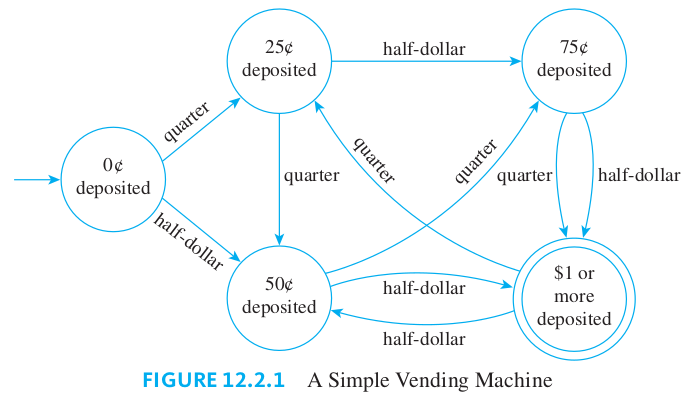
\includegraphics[scale=0.4]{../images/12.2.1.png}
\end{figure}

\subsubsection{(a)}
Quarter, half-dollar, quarter
\begin{proof}
\$1 or more deposited
\end{proof}

\subsubsection{(b)}
Quarter, half-dollar, half-dollar
\begin{proof}
\$1 or more deposited
\end{proof}

\subsubsection{(c)}
Half-dollar, quarter, quarter, quarter, half-dollar
\begin{proof}
75\textcentoldstyle{} or more deposited
\end{proof}

{\bf \cy In \(2-7\), a finite-state automaton is given by a transition diagram. For each automaton: \\
a. Find its states. \\
b. Find its input symbols. \\
c. Find its initial state. \\
d. Find its accepting states. \\
e. Write its annotated next-state table.}

\subsection{Exercise 2}
\begin{figure}[ht!]
\centering
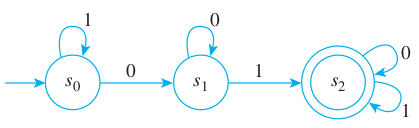
\includegraphics[scale=0.5]{../images/12.2.2.png}
\end{figure}

\begin{proof}
(a) \(s_0, s_1, s_2\) \,\,\, (b) 0, 1 \,\,\, (c) \(s_0\) \,\,\, (d) \(s_2\) 
(e) 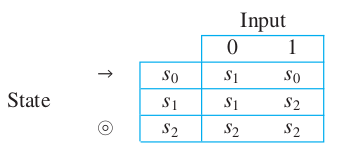
\includegraphics[scale=0.5]{../images/12.2.2.e.png}
\end{proof}

\subsection{Exercise 3}
\begin{figure}[ht!]
\centering
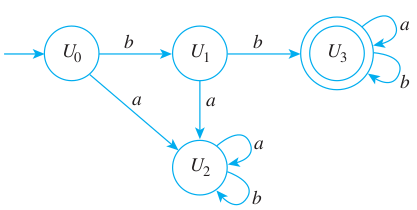
\includegraphics[scale=0.5]{../images/12.2.3.png}
\end{figure}

\begin{proof}
(a) \(U_0, U_1, U_2, U_3\) \,\, (b) \(a, b\) \,\, (c) \(U_0\) \,\, (d) \(U_3\) \,\, (e) 
\arrayrulecolor{cyan}
\begin{tabular}{|c|c|c|c|}
\hline
\(\) & \(\) & \(a\) & \(b\) \\
\hline
\(\to\) & \(U_0\) & \(U_2\) & \(U_1\) \\
\hline
\(\) & \(U_1\) & \(U_2\) & \(U_3\) \\
\hline
\(\) & \(U_2\) & \(U_2\) & \(U_2\) \\
\hline
\(\circ\) & \(U_3\) & \(U_3\) & \(U_3\) \\
\hline
\end{tabular}
\arrayrulecolor{black} % change it back!
\end{proof}

\subsection{Exercise 4}
\begin{figure}[ht!]
\centering
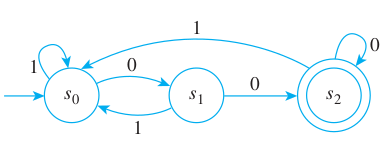
\includegraphics[scale=0.5]{../images/12.2.4.png}
\end{figure}

\begin{proof}
(a) \(s_0, s_1, s_2\) \,\, (b) \(0, 1\) \,\, (c) \(s_0\) \,\, (d) \(s_2\) \,\, (e) 
\arrayrulecolor{cyan}
\begin{tabular}{|c|c|c|c|}
\hline
\(\) & \(\) & \(a\) & \(b\) \\
\hline
\(\to\) & \(s_0\) & \(s_1\) & \(s_0\) \\
\hline
\(\) & \(s_1\) & \(s_2\) & \(s_0\) \\
\hline
\(\circ\) & \(s_2\) & \(s_2\) & \(s_0\) \\
\hline
\end{tabular}
\arrayrulecolor{black} % change it back!
\end{proof}

\subsection{Exercise 5}
\begin{figure}[ht!]
\centering
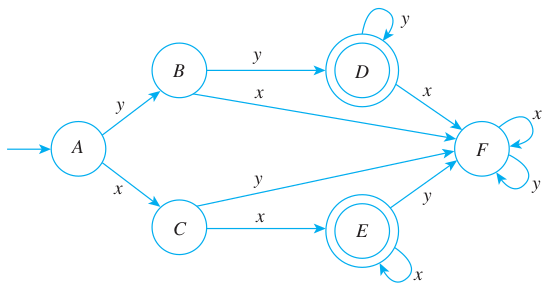
\includegraphics[scale=0.5]{../images/12.2.5.png}
\end{figure}

\begin{proof}
(a) \(A, B, C, D, E, F\) \,\, (b) \(x, y\) \,\, (c) \(A\) \,\, 
(d) \(D, E\) \,\, (e)
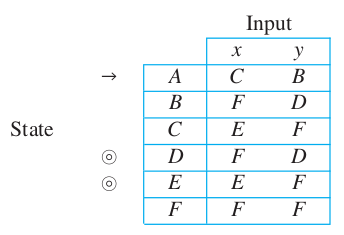
\includegraphics[scale=0.5]{../images/12.2.5.e.png}
\end{proof}

\subsection{Exercise 6}
\begin{figure}[ht!]
\centering
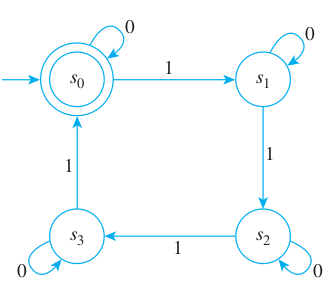
\includegraphics[scale=0.5]{../images/12.2.6.png}
\end{figure}

\begin{proof}
(a) \(s_0, s_1, s_2, s_3\) \,\, (b) \(0, 1\) \,\, (c) \(s_0\) \,\, (d) \(s_0\) \,\, (e) 
\arrayrulecolor{cyan}
\begin{tabular}{|c|c|c|c|}
\hline
\(\) & \(\) & \(0\) & \(1\) \\
\hline
\(\to \circ\) & \(s_0\) & \(s_0\) & \(s_1\) \\
\hline
\(\) & \(s_1\) & \(s_1\) & \(s_2\) \\
\hline
\(\) & \(s_2\) & \(s_2\) & \(s_3\) \\
\hline
\(\) & \(s_3\) & \(s_3\) & \(s_0\) \\
\hline
\end{tabular}
\arrayrulecolor{black} % change it back!
\end{proof}

\subsection{Exercise 7}
\begin{figure}[ht!]
\centering
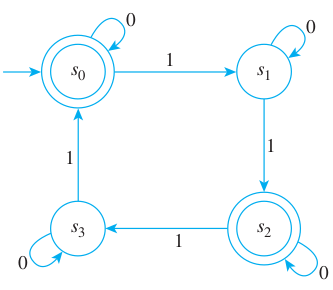
\includegraphics[scale=0.5]{../images/12.2.7.png}
\end{figure}

\begin{proof}
(a) \(s_0, s_1, s_2, s_3\) \,\, (b) 0, 1 \,\, (c) \(s_0\) \,\, 
(d) \(s_0, s_2\) \,\, (e)
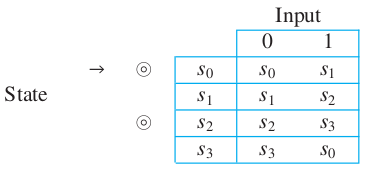
\includegraphics[scale=0.5]{../images/12.2.7.e.png}
\end{proof}

{\bf \cy In 8 and 9, a finite-state automaton is given by an annotated next-state table. For each automaton: \\
a. Find its states. \\
b. Find its input symbols. \\
c. Find its initial state. \\
d. Find its accepting states. \\
e. Draw its transition diagram.}

\subsection{Exercise 8}
\begin{figure}[ht!]
\centering
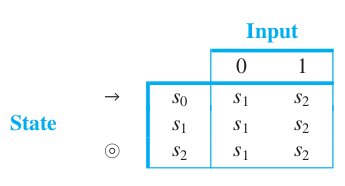
\includegraphics[scale=0.5]{../images/12.2.8.png}
\end{figure}

\begin{proof}
(a) \(s_0, s_1, s_2\) \,\, (b) 0, 1 \,\, (c) \(s_0\) \,\, (d) \(s_2\) \,\, (e)
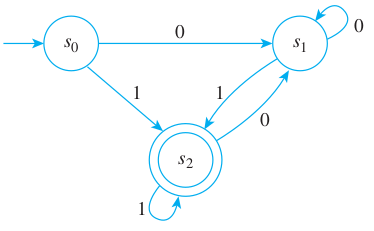
\includegraphics[scale=0.5]{../images/12.2.8.e.png}
\end{proof}

\subsection{Exercise 9}
\begin{figure}[ht!]
\centering
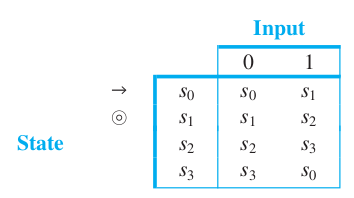
\includegraphics[scale=0.5]{../images/12.2.9.png}
\end{figure}

\begin{proof}
(a) \(s_0, s_1, s_2, s_3\) \,\, (b) 0, 1 \,\, (c) \(s_0\) \,\, (d) \(s_1\) \,\, 

(e) 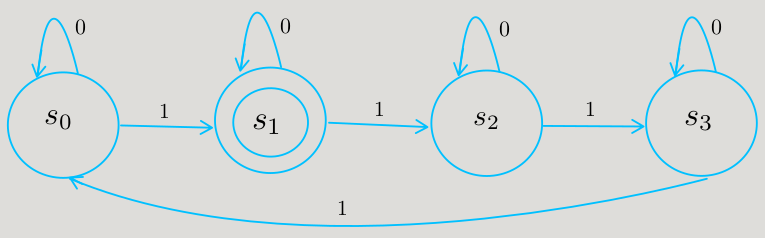
\includegraphics[scale=0.4]{../images/12.2.9.e.png}
\end{proof}

\subsection{Exercise 10}
A finite-state automaton \(A\), given by the transition diagram below, has next-state function \(N\) and eventual-
state function \(N^*\).

\begin{figure}[ht!]
\centering
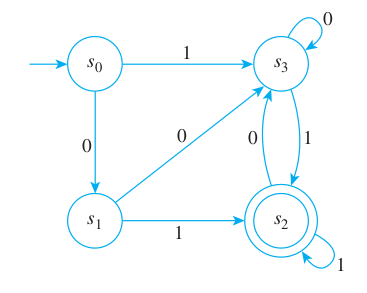
\includegraphics[scale=0.5]{../images/12.2.10.png}
\end{figure}

\subsubsection{(a)}
Find \(N(s_1, 1)\) and \(N(s_0, 1)\).
\begin{proof}
\(N(s_1, 1) = s_2, N(s_0, 1) = s_3\)
\end{proof}

\subsubsection{(b)}
Find \(N(s_2, 0)\) and \(N(s_1, 0)\).
\begin{proof}
\(N(s_2, 0) = s_3\) and \(N(s_1, 0) = s_3\)
\end{proof}

\subsubsection{(c)}
Find \(N^*(s_0, 10011)\) and \(N^*(s_1, 01001)\).
\begin{proof}
\(N^*(s_0, 10011) = s_2, N^*(s_1, 01001) = s_2\)
\end{proof}


\subsubsection{(d)}
Find \(N^*(s_2, 11010)\) and \(N^*(s_0, 01000)\).
\begin{proof}
\(N^*(s_2, 11010) = s_3\) and \(N^*(s_0, 01000) = s_3\).
\end{proof}


\subsection{Exercise 11}
A finite-state automaton \(A\), given by the transition diagram below, has next-state function \(N\) and eventual-
state function \(N^*\).

\begin{figure}[ht!]
\centering
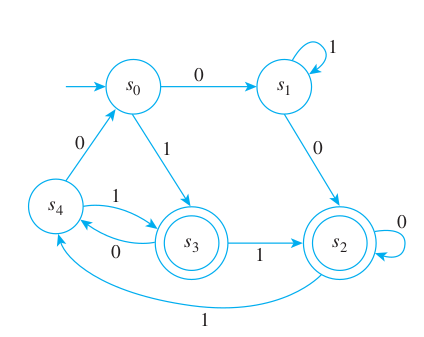
\includegraphics[scale=0.5]{../images/12.2.11.png}
\end{figure}

\subsubsection{(a)}
Find \(N(s_3, 0)\) and \(N(s_2, 1)\).
\begin{proof}
\(N(s_3, 0) = s_4, N(s_2, 1) = s_4\)
\end{proof}

\subsubsection{(b)}
Find \(N(s_0, 0)\) and \(N(s_4, 1)\).
\begin{proof}
\(N(s_0, 0) = s_1\) and \(N(s_4, 1) = s_3\).
\end{proof}

\subsubsection{(c)}
Find \(N^*(s_0, 010011)\) and \(N^*(s_3, 01101)\).
\begin{proof}
\(N^*(s_0, 010011) = s_3, N^*(s_3, 01101) = s_4\)
\end{proof}

\subsubsection{(d)}
Find \(N^*(s_0, 1111)\) and \(N^*(s_2, 00111)\).
\begin{proof}
\(N^*(s_0, 1111) = s_3\) and \(N^*(s_2, 00111) = s_2\).
\end{proof}

{\bf \cy Note that multiple correct answers exist for part (d) of exercises 12 and 13, part (b) of exercises \(14-19\), and 
for exercises \(20-48\).}

\subsection{Exercise 12}
Consider again the finite-state automaton of exercise 2.

\subsubsection{(a)}
To what state does the automaton go when the symbols of the following strings are input to it in sequence, starting from 
the initial state? 

(i) 1110001 (ii) 0001000 (iii) 11110000

\begin{proof}
(i) \(s_2\) (ii) \(s_2\) (iii) \(s_1\)
\end{proof}

\subsubsection{(b)}
Which of the strings in part (a) send the automaton to an accepting state?

\begin{proof}
those in (i) and (ii) but not (iii)
\end{proof}

\subsubsection{(c)}
What is the language accepted by the automaton?
\begin{proof}
The language accepted by this automaton is the set of all strings of 0’s and 1’s that contain at least one 0 followed 
(not necessarily immediately) by at least one 1.
\end{proof}

\subsubsection{(d)}
Find a regular expression that defines the language.
\begin{proof}
\(1^*00^*1(0 | 1)^*\)
\end{proof}

\subsection{Exercise 13}
Consider again the finite-state automaton of exercise 3.

\subsubsection{(a)}
To what state does the automaton go when the symbols of the following strings are input to it in sequence, starting from 
the initial state? 

(i) \(bb\) (ii) \(aabbbaba\) (iii) \(babbbbbabaa\) (iv) \(bbaaaabaa\)

\begin{proof}
(i) \(U_3\) (ii) \(U_2\) (iii) \(U_2\) (iv) \(U_3\)
\end{proof}

\subsubsection{(b)}
Which of the strings in part (a) send the automaton to an accepting state?

\begin{proof}
those in (i) and (iv) but not (ii) or (iii)
\end{proof}

\subsubsection{(c)}
What is the language accepted by the automaton?

\begin{proof}
All strings of \(a\)'s and \(b\)'s starting with at least two \(b\)'s.
\end{proof}

\subsubsection{(d)}
Find a regular expression that defines the language.

\begin{proof}
\(bb(a|b)^*\)
\end{proof}

{\bf \cy In each of \(14-19\), (a) find the language accepted by the automaton in the referenced exercise, and (b) find a 
regular expression that defines the same language.}

\subsection{Exercise 14}
Exercise 4

\subsubsection{(a)}
\begin{proof}
The language accepted by this automaton is the set of all strings of 0’s and 1’s that end in 00.
\end{proof}

\subsubsection{(b)}
\begin{proof}
\((0 | 1)^*00\)
\end{proof}

\subsection{Exercise 15}
Exercise 5
\subsubsection{(a)}
\begin{proof}
The language accepted by this automaton is the set of all strings of \(x\)’s and \(y\)’s of length at least two that 
consist either entirely of \(x\)’s or entirely of \(y\)’s.
\end{proof}

\subsubsection{(b)}
\begin{proof}
\(xxx^* | yyy^*\)
\end{proof}

\subsection{Exercise 16}
Exercise 6
\subsubsection{(a)}
\begin{proof}
The language accepted by this automaton is the set of all strings of 0’s and 1’s where the number of 1's is a multiple 
of 4. (This includes when the number of 1's is zero, i.e. strings consisting only of 0's.)
\end{proof}

\subsubsection{(b)}
\begin{proof}
\(0^* | (0^*10^*10^*10^*10^*)^*\)
\end{proof}

\subsection{Exercise 17}
Exercise 7
\subsubsection{(a)}
\begin{proof}
The language accepted by this automaton is the set of all strings of 0’s and 1’s with the following property: If \(n\) 
is the number of 1’s in the string, then \(n \mod 4 = 0\) or \(n \mod 4 = 2\). 
This is equivalent to saying that \(n\) is even.
\end{proof}

\subsubsection{(b)}
\begin{proof}
\(0^* | (0^*10^*10^*)^*\)
\end{proof}

\subsection{Exercise 18}
Exercise 8
\subsubsection{(a)}

\begin{proof}
The language accepted by this automaton is the set of all strings of 0’s and 1’s that end in 1.
\end{proof}

\subsubsection{(b)}

\begin{proof}
\((0 | 1)^*1\)
\end{proof}

\subsection{Exercise 19}
Exercise 9
\subsubsection{(a)}

\begin{proof}
The language accepted by this automaton is set of all strings of 0’s and 1’s, with the property that if \(n\) is the number
of 1's in the string, then \(n \mod 4 = 1\).
\end{proof}

\subsubsection{(b)}

\begin{proof}
\((0^*10^*10^*10^*1)^*1(0^*10^*10^*10^*1)^*\)
\end{proof}

{\bf \cy In each of \(20-28\), (a) design an automaton with the given input alphabet that accepts the given set of 
strings, and (b) find a regular expression that defines the language accepted by the automaton.}

\subsection{Exercise 20}
Input alphabet \(= \{0, 1\}\); Accepts the set of all strings for which the final three input symbols are 1.

\subsubsection{(a)}

\begin{proof}
Call the automaton being constructed \(A\). Acceptance of a string by \(A\) depends on the values of three consecutive 
inputs. Thus \(A\) requires at least four states: \\
\(s_0\): initial state \\
\(s_1\): state indicating that the last input character was a 1 \\
\(s_2\): state indicating that the last two input characters were 1’s \\
\(s_3\): state indicating that the last three input characters were 1’s, the acceptance state

If \(a_0\) is input to \(A\) when it is in state \(s_0\), no progress is made toward achieving a string of three 
consecutive 1’s. Hence \(A\) should remain in state \(s_0\). If \(a_1\) is input to \(A\) when it is in state \(s_0\), it 
goes to state \(s_1\), which indicates that the last input 
character of the string is a 1. From state \(s_1\), \(A\) goes to state \(s_2\) if a 1 is input. This indicates that the last 
two characters of the string are 1’s. But if \(a_0\) is input, \(A\) should return to \(s_0\) because the wait for a string 
of three consecutive 1’s must start over again. When \(A\) is in state \(s_2\) and a 1 is input, then a string of three 
consecutive 1’s is achieved, so \(A\) should go to state \(s_3\). If a 0 is input when \(A\) is in state \(s_2\), then 
progress toward accumulating a sequence of three consecutive 1’s is lost, so \(A\) should return to \(s_0\). When \(A\) is 
in a state \(s_3\) and a 1 is input, then the final three symbols of the input string are 1’s, and so \(A\) should stay 
in state \(s_3\). If a 0 is input when \(A\) is in state \(s_3\), then \(A\) should return to state \(s_0\) to await the
input of more 1’s. Thus the transition diagram is as follows:

\begin{figure}[ht!]
\centering
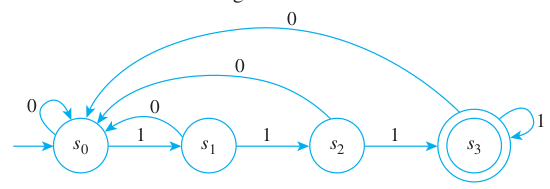
\includegraphics[scale=0.5]{../images/12.2.20.a.png}
\end{figure}
\end{proof}

\subsubsection{(b)}
\begin{proof}
\((0|1)*111\)
\end{proof}

\subsection{Exercise 21}
Input alphabet \(= \{0, 1\}\); Accepts the set of all strings that start with 01.

\subsubsection{(a)}

\begin{proof}
\begin{figure}[ht!]
\centering
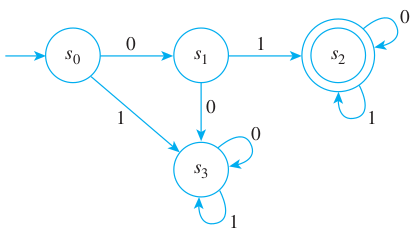
\includegraphics[scale=0.5]{../images/12.2.21.a.png}
\end{figure}
\end{proof}

\subsubsection{(b)}

\begin{proof}
\(01(0 | 1)^*\)
\end{proof}

\subsection{Exercise 22}
Input alphabet \(= \{a, b\}\); Accepts the set of all strings of length at least 2 for which the final two input symbols are 
the same.

\subsubsection{(a)}
\begin{proof}
Use five states: \(s_0\) (the initial state), \(s_1\) (the state indicating that the previous input symbol was an \(a\)), 
\(s_2\) (the state indicating that the previous input symbol was a \(b\)), \(s_3\) (the state indicating that the previous 
two input symbols were \(a\)’s), and \(s_4\) (the state indicating that the previous two input symbols were \(b\)’s).

\begin{figure}[ht!]
\centering
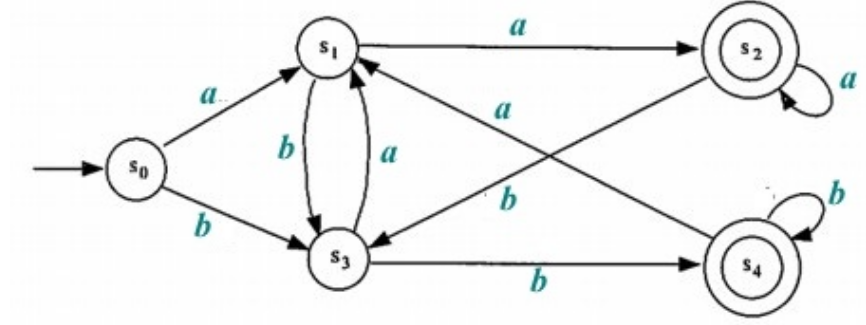
\includegraphics[scale=0.3]{../images/12.2.22.a.png}
\end{figure}
\end{proof}

\subsubsection{(b)}
\begin{proof}
\((a|b)^*(aa|bb)\)
\end{proof}

\subsection{Exercise 23}
Input alphabet \(= \{0, 1\}\); Accepts the set of all strings that start with 01 or 10.

\subsubsection{(a)}
\begin{proof}
\begin{figure}[ht!]
\centering
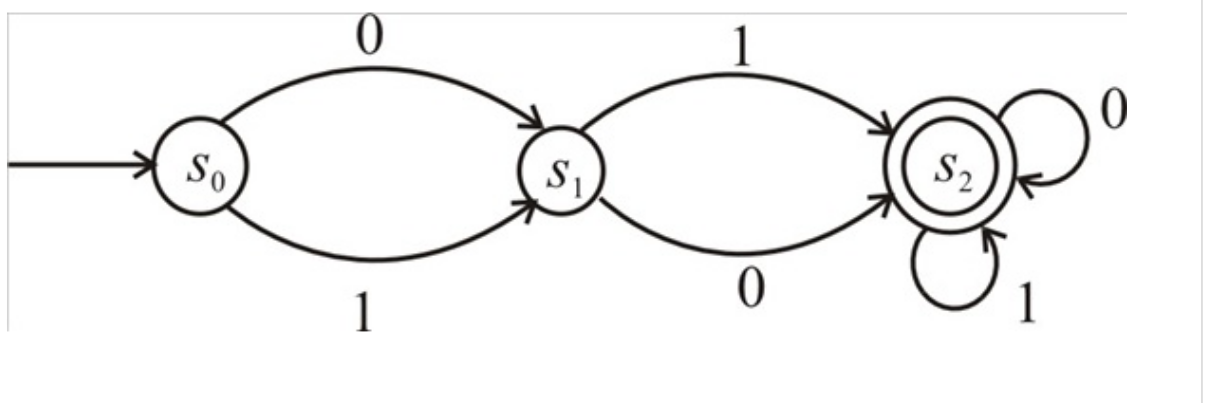
\includegraphics[scale=0.3]{../images/12.2.23.a.png}
\end{figure}
\end{proof}

\subsubsection{(b)}
\begin{proof}
\((01|10)(0|1)^*\)
\end{proof}

\subsection{Exercise 24}
Input alphabet \(= \{0, 1\}\); Accepts the set of all strings that start with 101.

\subsubsection{(a)}

\begin{proof}
\begin{figure}[ht!]
\centering
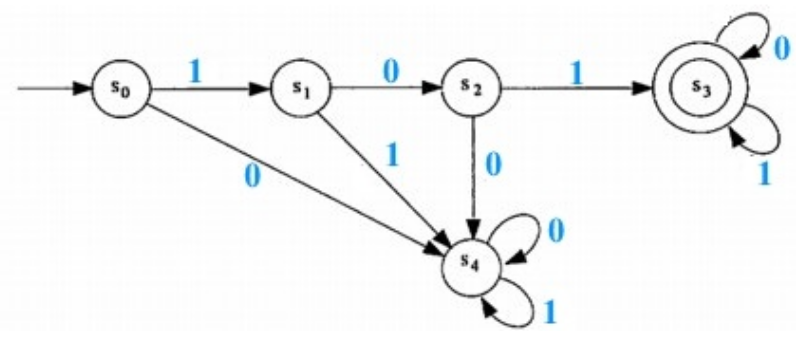
\includegraphics[scale=0.4]{../images/12.2.24.a.png}
\end{figure}
\end{proof}

\subsubsection{(b)}

\begin{proof}
\(101(0|1)^*\)
\end{proof}

\subsection{Exercise 25}
Input alphabet \(= \{0, 1\}\); Accepts the set of all strings that end in 10.

\subsubsection{(a)}
\begin{proof}
\begin{figure}[ht!]
\centering
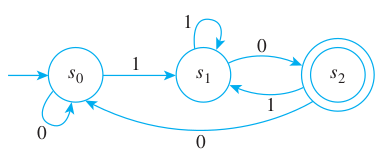
\includegraphics[scale=0.5]{../images/12.2.25.a.png}
\end{figure}
\end{proof}

\subsubsection{(b)}
\begin{proof}
\((0|1)^*10\)
\end{proof}

\subsection{Exercise 26}
Input alphabet \(= \{a, b\}\); Accepts the set of all strings that contain exactly two \(b\)’s.

\subsubsection{(a)}
\begin{proof}
\begin{figure}[ht!]
\centering
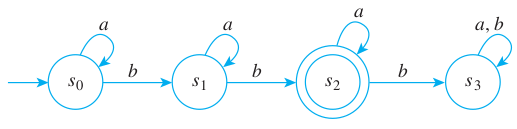
\includegraphics[scale=0.5]{../images/12.2.26.a.png}
\end{figure}
\end{proof}

\subsubsection{(b)}
\begin{proof}
\(a^*ba^*ba^*\)
\end{proof}

\subsection{Exercise 27}
Input alphabet \(= \{0, 1\}\); Accepts the set of all strings that start with 0 and contain exactly one 1.

\subsubsection{(a)}
\begin{proof}
\begin{figure}[ht!]
\centering
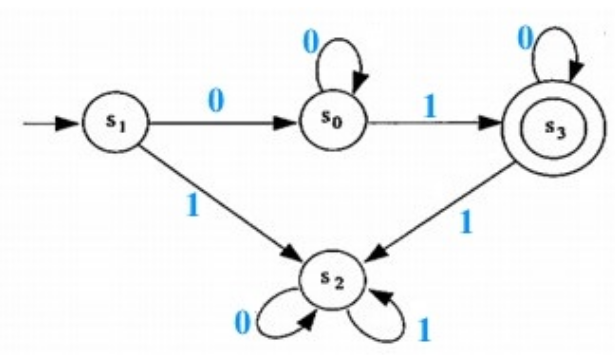
\includegraphics[scale=0.4]{../images/12.2.27.a.png}
\end{figure}
\end{proof}

\subsubsection{(b)}
\begin{proof}
\(00^*10^*\)
\end{proof}

\subsection{Exercise 28}
Input alphabet \(= \{0, 1\}\); Accepts the set of all strings that contain the pattern 010.

\subsubsection{(a)}
\begin{proof}
\begin{figure}[ht!]
\centering
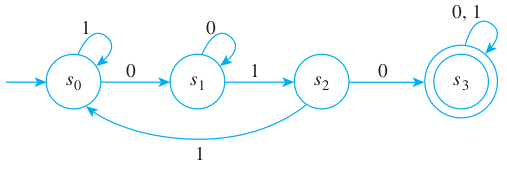
\includegraphics[scale=0.5]{../images/12.2.28.a.png}
\end{figure}
\end{proof}

\subsubsection{(b)}
\begin{proof}
\((0|1)^*101(0|1)^*\)
\end{proof}

{\bf \cy In \(29-47\), design a finite-state automaton to accept the language defined by the regular expression in the 
referenced exercise from Section 12.1.}

\subsection{Exercise 29}
Exercise 16: \(0^*1(0^*1^*)^*\)
\begin{proof}
\begin{figure}[ht!]
\centering
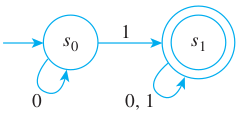
\includegraphics[scale=0.5]{../images/12.2.29.png}
\end{figure}
\end{proof}

\subsection{Exercise 30}
Exercise 17: \(b^* | b^*ab^*\)
\begin{proof}
\begin{figure}[ht!]
\centering
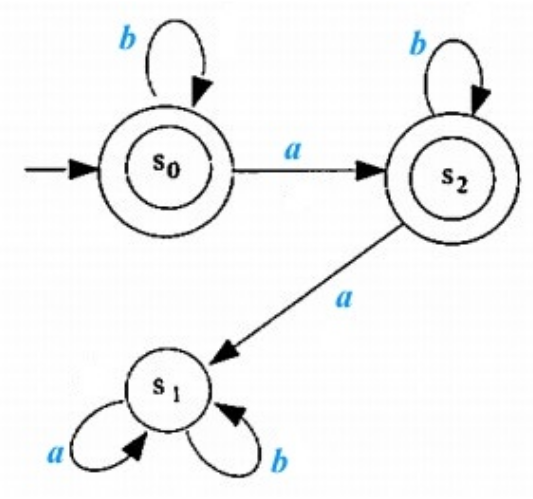
\includegraphics[scale=0.3]{../images/12.2.30.png}
\end{figure}
\end{proof}

\subsection{Exercise 31}
Exercise 18: \(x^*(yxxy | x)^*\)
\begin{proof}
Errata says: add two arrow loops from \(s_4\) to itself, one for \(x\) and one for \(y\).

\begin{figure}[ht!]
\centering
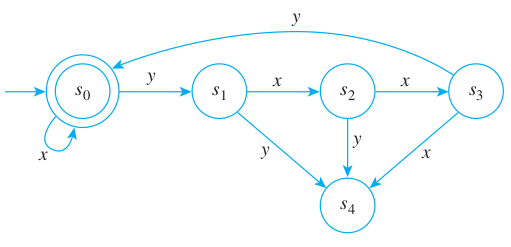
\includegraphics[scale=0.5]{../images/12.2.31.png}
\end{figure}
\end{proof}

\subsection{Exercise 32}
Exercise 19: \(b^*ab^*ab^*a\)
\begin{proof}
\begin{figure}[ht!]
\centering
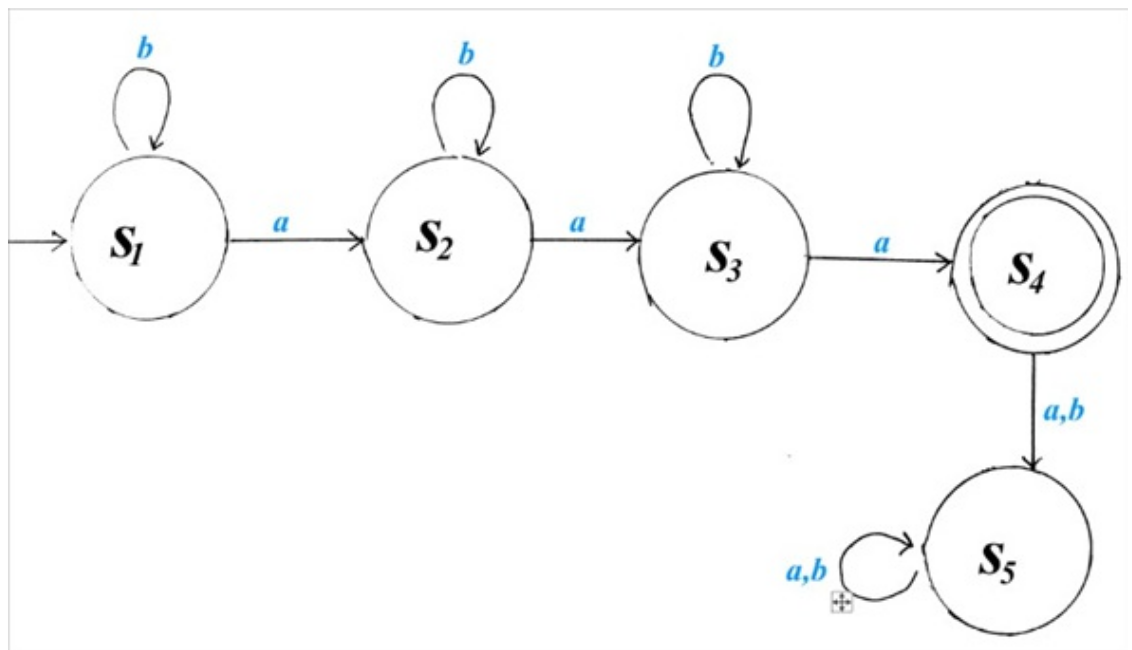
\includegraphics[scale=0.2]{../images/12.2.32.png}
\end{figure}
\end{proof}

\subsection{Exercise 33}
Exercise 20: \(1(0 | 1)^* 00\)
\begin{proof}
\begin{figure}[ht!]
\centering
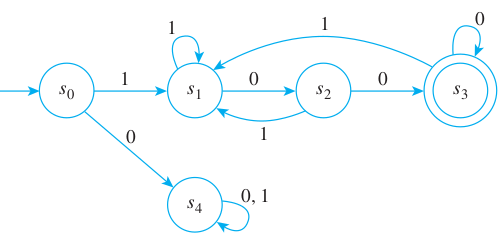
\includegraphics[scale=0.5]{../images/12.2.33.png}
\end{figure}
\end{proof}

\subsection{Exercise 34}
Exercise 21: \((x | y)y(x | y)^*\)
\begin{proof}
\begin{figure}[ht!]
\centering
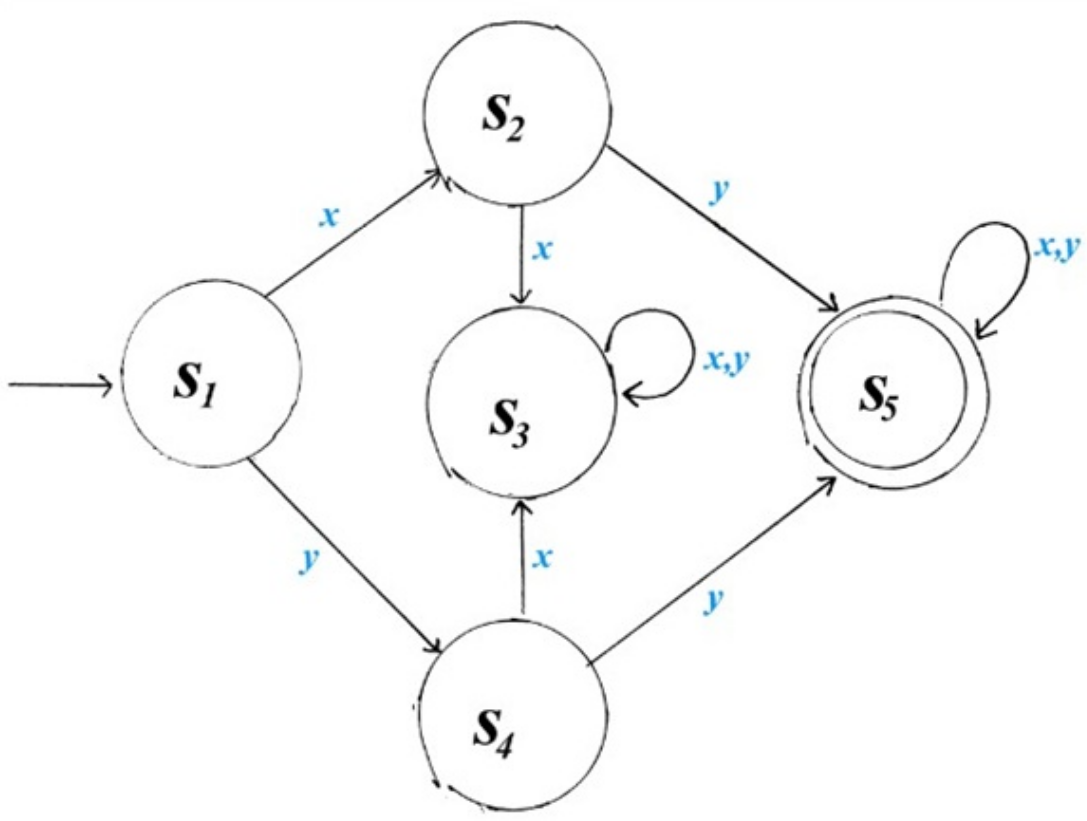
\includegraphics[scale=0.2]{../images/12.2.34.png}
\end{figure}
\end{proof}

\subsection{Exercise 35}
Exercise 24: \((01^*2)^*\)
\begin{proof}
\begin{figure}[ht!]
\centering
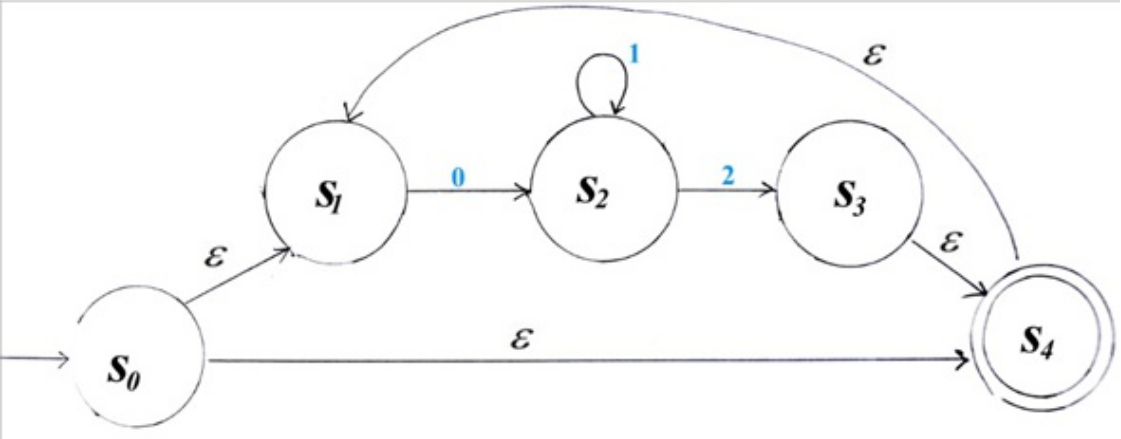
\includegraphics[scale=0.3]{../images/12.2.35.png}
\end{figure}
\end{proof}

\subsection{Exercise 36}
Exercise 25: \(0^*10^*(0^*10^*10^*)^*\).
\begin{proof}
\begin{figure}[ht!]
\centering
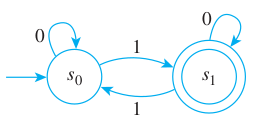
\includegraphics[scale=0.5]{../images/12.2.36.png}
\end{figure}
\end{proof}

\subsection{Exercise 37}
Exercise 26: \((a|b)^*b(aa|ab|ba|bb)\)
\begin{proof}
\begin{figure}[ht!]
\centering
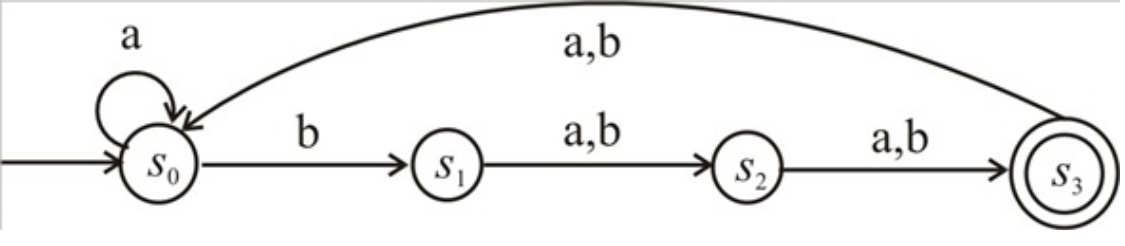
\includegraphics[scale=0.3]{../images/12.2.37.png}
\end{figure}
\end{proof}

\subsection{Exercise 38}
Exercise 27: \(y^*(xyy^*)^*(\lambda | x)\).
\begin{proof}
\begin{figure}[ht!]
\centering
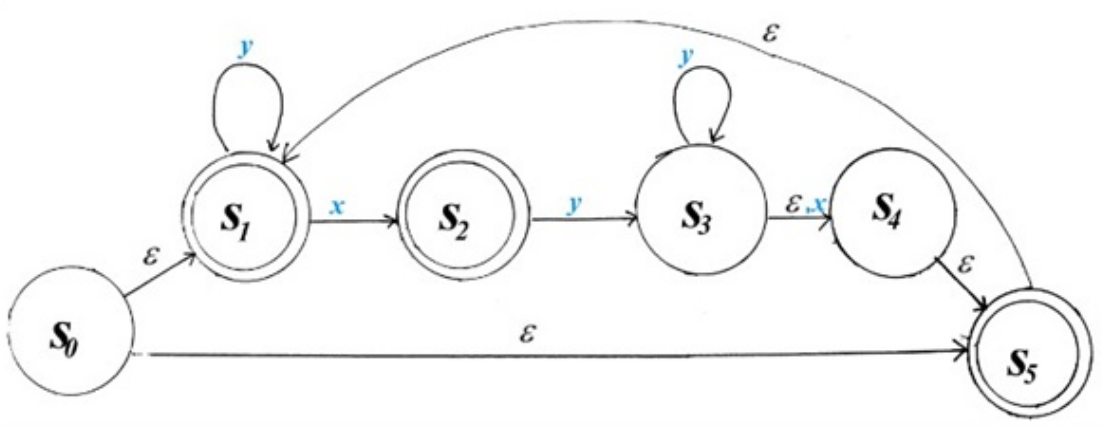
\includegraphics[scale=0.3]{../images/12.2.38.png}
\end{figure}
\end{proof}

\subsection{Exercise 39}
Exercise 31:  \(pre[a - z]^+\)
\begin{proof}
Let \(\hat{P}\) denote a list of all letters of a lowercase alphabet except \(p\), \(\hat{R}\) denote a list of all the 
letters of a lowercase alphabet except \(r\), and \(\hat{E}\) denote a list of all the letters of a lowercase alphabet 
except \(e\).

\begin{figure}[ht!]
\centering
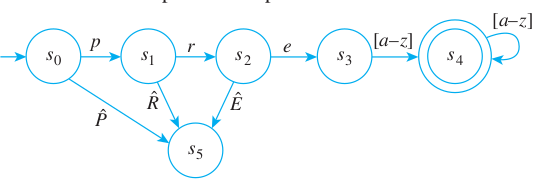
\includegraphics[scale=0.5]{../images/12.2.39.png}
\end{figure}
\end{proof}

\subsection{Exercise 40}
Exercise 32: \([A-Z]^*(BIO | INFO)[A-Z]^*\)
\begin{proof}
\begin{figure}[ht!]
\centering
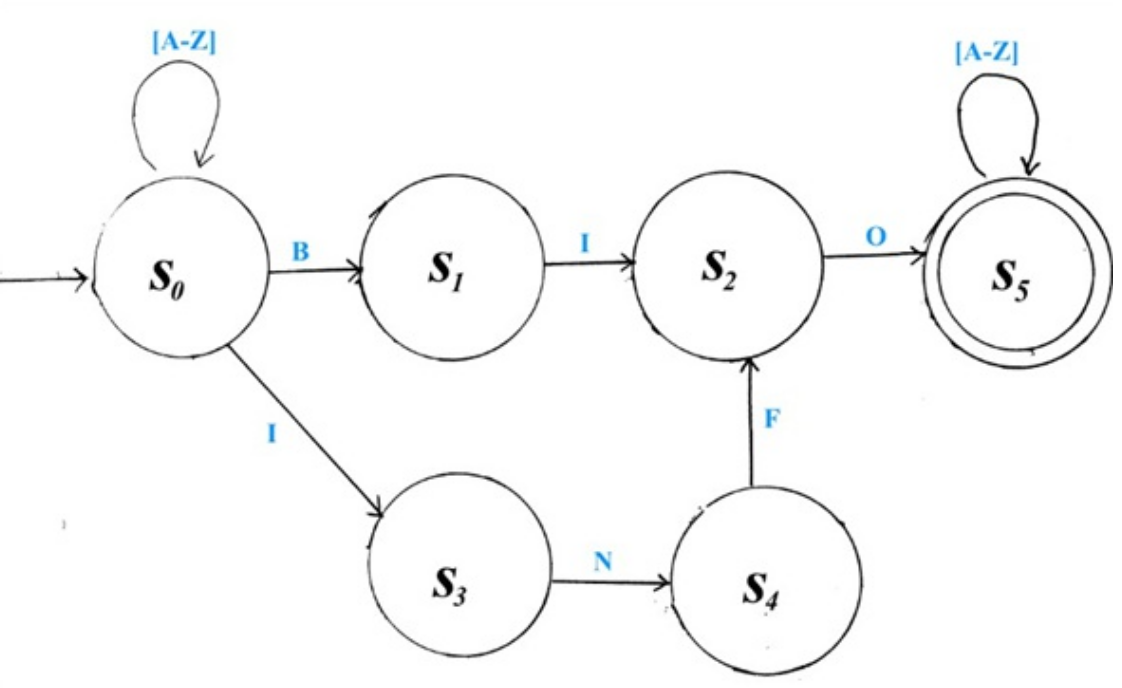
\includegraphics[scale=0.25]{../images/12.2.40.png}
\end{figure}
\end{proof}

\subsection{Exercise 41}
Exercise 33: \([a-z]^+[a-z]^+[a-z]^+ ly\)
\begin{proof}
\begin{figure}[ht!]
\centering
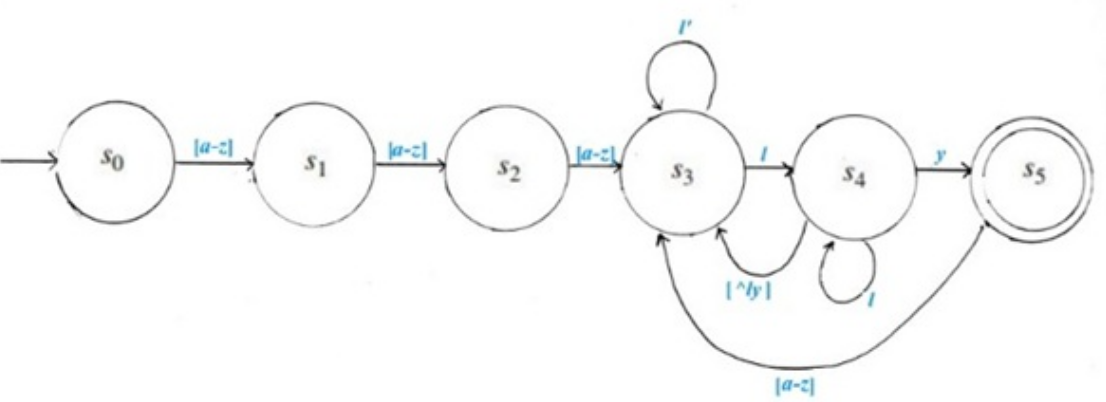
\includegraphics[scale=0.4]{../images/12.2.41.png}
\end{figure}
\end{proof}

\subsection{Exercise 42}
Exercise 34: \([a - z]^*(a | e | i | o | u)[a - z]^*\)
\begin{proof}
Let \(\mathscr{S}\) denote a list of all the consonants in a lowercase alphabet.

\begin{figure}[ht!]
\centering
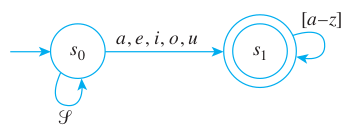
\includegraphics[scale=0.5]{../images/12.2.42.png}
\end{figure}
\end{proof}

\subsection{Exercise 43}
Exercise 35: \([\string^ aeiou]^*(a|e|i|o|u)[\string^ aeiou]^*\)
\begin{proof}
{\it ???}
\end{proof}

\subsection{Exercise 44}
Exercise 36: \([\string^ AEIOU][A-Z]^*[AEIOU]\{2\}[A-Z]^*\)
\begin{proof}
{\it ???}
\end{proof}

\subsection{Exercise 45}
Exercise 37: \([0 - 9]\{3\} - [0 - 9]\{2\} - 3[0 - 9]\{2\}6\)
\begin{proof}
\begin{figure}[ht!]
\centering
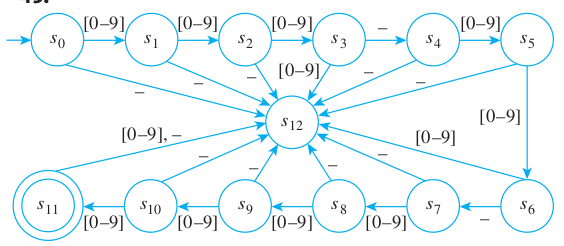
\includegraphics[scale=0.5]{../images/12.2.45.png}
\end{figure}
\end{proof}

\subsection{Exercise 46}
Exercise 38: \((800|888)-[0-9]\{3\}-2[0-9]\{2\}2\)
\begin{proof}
{\it ???}
\end{proof}

\subsection{Exercise 47}
Exercise 39: \(([+ -] | \lambda)[0 - 9]^* (\backslash. | \lambda)[0 - 9]^*\)
\begin{proof}
{\it ???}
\end{proof}

\subsection{Exercise 48}
A simplified telephone switching system allows the following strings as legal telephone numbers. Design a finite-state 
automaton to recognize all the legal telephone numbers in (a), (b), and (c). Include an “error state” for invalid telephone 
numbers.

\subsubsection{(a)}
A string of seven digits in which neither of the first two digits is a 0 or 1 (a local call string).

\begin{proof}
A regular expression is \([2-9]{2}[0-9]{5}\).
\end{proof}

\subsubsection{(b)}
A 1 followed by a three-digit area code string (any digit except 0 or 1 followed by a 0 or 1 followed by any digit) 
followed by a seven-digit local call string.

\begin{proof}
A regular expression is \(1[2-9](0|1)[0-9][2-9]{2}[0-9]{5}\). Here we are using the regular expression from part (a) for the
local call string.
\end{proof}

\subsubsection{(c)}
A 0 alone or followed by a three-digit area code string plus a seven-digit local call string.

\begin{proof}
A regular expression is \(0(([2-9](0|1)[0-9])?)[2-9]{2}[0-9]{5}\) (using the local call string and the area code string).
\end{proof}

\subsection{Exercise 49}
Write a computer algorithm that simulates the action of the finite-state automaton of exercise 2 by mimicking the action 
of the transition diagram.

\begin{proof}
{\it ???}
\end{proof}

\subsection{Exercise 50}
Write a computer algorithm that simulates the action of the finite-state automaton of exercise 8 by repeated application 
of the next-state function.

\begin{proof}
{\it ???}
\end{proof}

\subsection{Exercise 51}
Let \(L\) be the language consisting of all strings of the form \(a^mb^n\), where \(m\) and \(n\) are positive integers 
and \(m \geq n\). Show that there is no finite-state automaton that accepts \(L\).

\begin{proof}
This proof is virtually identical to that of Example 12.2.8. Just take \(p\) and \(q\) in that proof so that \(p > q\). 
From the fact that \(A\) accepts \(a^pb^p\), you can deduce that \(A\) accepts \(a^qb^p\). Since \(p > q\), this string is 
not in \(L\).
\end{proof}

\subsection{Exercise 52}
Let \(L\) be the language consisting of all strings of the form \(a^mb^n\), where \(m\) and \(n\) are positive integers 
and \(m \leq n\). Show that there is no finite-state automaton that accepts \(L\).

\begin{proof}
{\it ???}
\end{proof}

\subsection{Exercise 53}
Let \(L\) be the language consisting of all strings of the form \(a^n\), where \(n = m^2\), for some positive integer 
\(m\). Show that there is no finite-state automaton that accepts \(L\).

\begin{proof}
Suppose the automaton \(A\) has \(N\) states. Choose an integer \(m\) such that \((m + 1)^2 - m^2 > N\). Consider 
strings of \(a\)’s of lengths between \(m^2\) and \((m + 1)^2\). Since there are more strings than states, at least two 
strings must send \(A\) to the same state \(s_i\):

\begin{figure}[ht!]
\centering
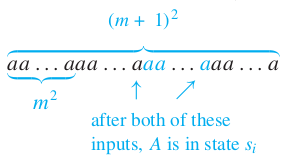
\includegraphics[scale=0.5]{../images/12.2.53.png}
\end{figure}

It follows (by removing the \(a\)’s shown in color) that the automaton must accept a string of the form \(a^k\), where 
\(m^2 < k < (m + 1)^2\).
\end{proof}

\subsection{Exercise 54}
\subsubsection{(a)}
Let \(A\) be a finite-state automaton with input alphabet \(\Sigma\), and suppose \(L(A)\) is the language accepted by 
\(A\). The complement of \(L(A)\) is the set of all strings over \(\Sigma\) that are not in \(L(A)\). Show that the 
complement of a regular language is regular by proving the following: If \(L(A)\) is the language accepted by a 
finite-state automaton \(A\), then there is a finite-state automaton \(A'\) that accepts the complement of \(L(A)\).

\begin{proof}
{\it ???}
\end{proof}

\subsubsection{(b)}
Show that the intersection of any two regular languages is regular as follows: First prove that if \(L(A_1)\) and 
\(L(A_2)\) are languages accepted by automata \(A_1\) and \(A_2\), respectively, then there is an automaton \(A\) that 
accepts \((L(A_1))^c \cup (L(A_2))^c\). Then use one of De Morgan’s laws for sets, the double complement law for sets, 
and the result of part (a) to prove that there is an automaton that accepts \(L(A_1) \cap L(A_2)\).

\begin{proof}
{\it ???}
\end{proof}

\section{Exercise Set 12.3}
\subsection{Exercise 1}

\subsubsection{(a)}

\begin{proof}
0-equivalence classes: \(\{s_0, s_1, s_3, s_4\}, \{s_2, s_5\}\) \\
1-equivalence classes: \(\{s_0, s_3\}, \{s_1, s_4\}, \{s_2, s_5\}\) \\
2-equivalence classes: \(\{s_0, s_3\}, \{s_1, s_4\}, \{s_2, s_5\}\) \\
\end{proof}

\subsubsection{(b)}

\begin{proof}
\begin{figure}[ht!]
\centering
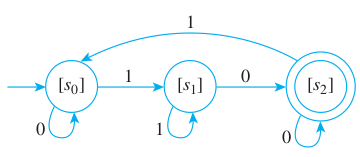
\includegraphics[scale=0.5]{../images/12.3.1.b.png}
\end{figure}
\end{proof}

\subsection{Exercise 2}

\subsubsection{()}

\begin{proof}

\end{proof}

\subsection{Exercise 3}

\subsubsection{()}

\begin{proof}

\end{proof}

\subsection{Exercise 4}

\subsubsection{(a)}

\begin{proof}
0-equivalence classes: \(\{s_0, s_1, s_2\}, \{s_3, s_4, s_5\}\) \\
1-equivalence classes: \(\{s_0, s_1, s_2\}, \{s_3, s_5\}, \{s_4\}\) \\
2-equivalence classes: \(\{s_0, s_2\}, \{s_1\}, \{s_3, s_5\}, \{s_4\}\) \\
3-equivalence classes: \(\{s_0, s_2\}, \{s_1\}, \{s_3, s_5\}, \{s_4\}\)
\end{proof}

\subsubsection{(b)}

\begin{proof}
\begin{figure}[ht!]
\centering
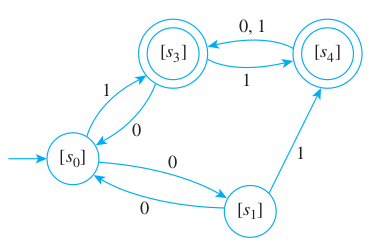
\includegraphics[scale=0.5]{../images/12.3.4.b.png}
\end{figure}
\end{proof}

\subsection{Exercise 5}

\subsubsection{()}

\begin{proof}

\end{proof}

\subsection{Exercise 6}

\subsubsection{(a)}

\begin{proof}
The 3-equivalence classes are \(\{s_0\}, \{s_1\}, \{s_2\}, \{s_3\}, \{s_4\}, \{s_5\}\), and \(\{s_6\}\).
\end{proof}

\subsubsection{(b)}

\begin{proof}

\end{proof}

\subsection{Exercise 7}

\subsubsection{()}

\begin{proof}
Yes. For A: \\
0-equivalence classes: \(\{s_0, s_2\}, \{s_1, s_3\}\) \\
1-equivalence classes: \(\{s_0\}, \{s_2\}, \{s_1, s_3\}\) \\
2-equivalence classes: \(\{s_0\}, \{s_2\}, \{s_1, s_3\}\)

Transition diagram for \(\overline{A}\):

\begin{figure}[ht!]
\centering
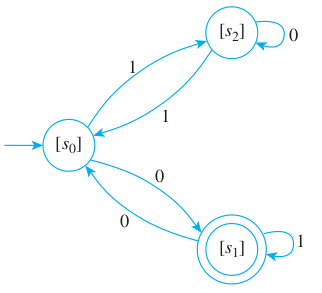
\includegraphics[scale=0.5]{../images/12.3.7.a.png}
\end{figure}

For \(A'\): \\
0-equivalence classes: \(\{s'_0, s'_1, s'_2\}, \{s'_3\}\) \\
1-equivalence classes: \(\{s'_0, s'_2\}, \{s'_1\}, \{s'_3\}\) \\
2-equivalence classes: \(\{s'_0, s'_2\}, \{s'_1\}, \{s'_3\}\)

Transition diagram for \(\overline{A'}\):

\begin{figure}[ht!]
\centering
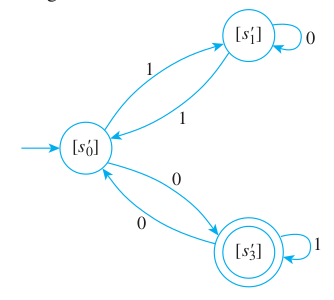
\includegraphics[scale=0.5]{../images/12.3.7.b.png}
\end{figure}

Except for the labeling of the states, the transition diagrams for \(A\) and \(A'\) are identical. Hence \(A\) and \(A\) 
accept the same language, and so, by Theorem 12.3.3, \(A\) and \(A'\) also accept the same language. Thus \(A\) and \(A'\) 
are equivalent automata.
\end{proof}

\subsection{Exercise 8}

\subsubsection{()}

\begin{proof}

\end{proof}

\subsection{Exercise 9}

\subsubsection{()}

\begin{proof}
For \(A\): \\
0-equivalence classes: \(\{s_1, s_2, s_4, s_5\}, \{s_0, s_3\}\) \\
1-equivalence classes: \(\{s_1, s_2\}, \{s_4, s_5\}, \{s_0, s_3\}\) \\
2-equivalence classes: \(\{s_1\}, \{s_2\}, \{s_4, s_5\}, \{s_0, s_3\}\) \\
3-equivalence classes: \(\{s_1\}, \{s_2\}, \{s_4, s_5\}, \{s_0, s_3\}\)

Therefore, the states of \(\overline{A}\) are the 3-equivalence classes of \(A\).

For \(A'\): \\
0-equivalence classes: \(\{s'_2, s'_3, s'_4, s'_5\}, \{s'_0, s'_1\}\) \\
1-equivalence classes: \(\{s'_2, s'_3, s'_4, s'_5\}, \{s'_0, s'_1\}\)

Therefore, the states of \(\overline{A'}\) are the 1-equivalence classes of \(A'\).

According to the text, two automata are equivalent if, and only if, their quotient automata are isomorphic, provided 
inaccessible states have first been removed. Now \(A\) and \(A'\) have no inaccessible states, and \(A\) has four states, 
whereas \(A'\) has only two states. Therefore, \(A\) and \(A'\) are not equivalent.

This result can also be obtained by noting, for example, that the string 11 is accepted by \(A'\) but not by \(A\).
\end{proof}

\subsection{Exercise 10}

\subsubsection{()}

\begin{proof}

\end{proof}

\subsection{Exercise 11}

\subsubsection{()}

\begin{proof}
{\it Partial answer:} Suppose \(A\) is a finite-state automaton with set of states \(S\) and relation \(R^*\) of 
\(*\)-equivalence of states. {\it [To show that \(R^*\) is an equivalence relation, we must show that \(R\) is reflexive, 
symmetric, and transitive.]}

{\bf Proof that \(R^*\) is symmetric:} {\it [We must show that for all states \(s\) and \(t\), if \(sR^*t\) then \(tR^*s\).]}

Suppose that \(s\) and \(t\) are any states of \(A\) such that \(sR^*t\). {\it [We must show that \(tR^*s\).]} Since 
\(sR^*t\), then for every input string \(w\),

\(N^*(s, w)\) is an accepting state \(\iff\) \(N^*(t, w)\) is an accepting state,

where \(N^*\) is the eventual-state function on \(A\). It follows from the symmetry of the \(\iff\) relation that for 
every input string \(w\), 

\(N^*(t, w)\) is an accepting state \(\iff\) \(N^*(s, w)\) is an accepting state.

Hence \(tR^*s\) {\it [as was to be shown]}, and so \(R^*\) is symmetric.
\end{proof}

\subsection{Exercise 12}

\subsubsection{()}

\begin{proof}
The proof is identical to the proof of property (12.3.1) given in the solution to exercise 11 provided every occurrence of 
“for each input string \(w\)” is replaced by “for each input string \(w\) of length less than or equal to \(k\).”
\end{proof}

\subsection{Exercise 13}

\subsubsection{()}

\begin{proof}
By property (12.3.2), for each integer \(k \geq 0\), \(k\)-equivalence is an equivalence relation. Now by Theorem 10.3.4, 
the distinct equivalence classes of an equivalence relation form a partition of the set on which the relation is defined. 
In this case, the relation is defined on the set of all states of the automaton. So the \(k\)-equivalence classes form a 
partition of the set of all states of the automaton.
\end{proof}

\subsection{Exercise 14}

\subsubsection{()}

\begin{proof}

\end{proof}

\subsection{Exercise 15}

\subsubsection{()}

\begin{proof}
Hint 1: Suppose Ck is a particular but arbitrarily chosen \(k\)-equivalence class. You must show that there is a 
\((k - 1)\)-equivalence class \(C_{k-1}\) such that \(C_k \subseteq C_{k-1}\).

If \(s\) is any element in \(C_k\), then \(s\) is a state of the automaton. Now the \((k - 1)\)-equivalence classes 
partition the set of all states of the automaton into a union of mutually disjoint subsets, so \(s \in C_{k-1}\) for some 
\((k - 1)\)-equivalence class \(C_{k-1}\).

To show that \(C_k \subseteq C_{k-1}\), you must show that for any state \(t\), if \(t \in C_k\), then \(t \in C_{k-1}\).
\end{proof}

\subsection{Exercise 16}

\subsubsection{()}

\begin{proof}

\end{proof}

\subsection{Exercise 17}

\subsubsection{()}

\begin{proof}
If \(m < k\), then every input string of length less than or equal to \(m\) has length less than or equal to \(k\).
\end{proof}

\subsection{Exercise 18}

\subsubsection{()}

\begin{proof}

\end{proof}

\subsection{Exercise 19}

\subsubsection{()}

\begin{proof}
Suppose two states \(s\) and \(t\) are equivalent. We must show that for any input symbol \(m\), the next-states 
\(N(s, m)\) and \(N(t, m)\) are equivalent. To do this, use the definition of equivalence and the fact that for any string 
\(w'\), input symbol \(m\), and state \(s\), \(N^*(N(s, m), w') = N^*(s, mw')\).
\end{proof}

\end{document}
